% !TEX root=exama-221012.tex
%--------------------------------------
% Create title frame
\titleframe

%--------------------------------------
% Table of contents
\begin{frame}{Overview}
  \setbeamertemplate{section in toc}[sections numbered]
  \tableofcontents[hideallsubsections]
\end{frame}


%==============================================
\section{Introduction}
\subsection{Tour de Table}
\begin{frame}
  \frametitle{\insertsectionhead}
  \framesubtitle{\insertsubsectionhead}

  \begin{itemize}
    \item CEA 
    \begin{itemize}
      \item DAM \textbf{Lydie Grospellier} (LG)
      \item DES \textbf{Vincent Faucher} (VF) \textbf{Isabelle Ramière} (IR)  
    \end{itemize}
    \item INRIA 
    \begin{itemize}
      \item Bordeaux \textbf{Hélène Barucq} (HB) \textbf{Luc Giraud} (LGi)
      \item  Grenoble \textbf{Arthur Vidard} (AV)
      \item Lille \textbf{El-Ghazali Talbi} (ET) Nourédine Melab (NM)
      \item Paris \textbf{Laura Grigori} (LG) \textbf{Frédéric Nataf} (FN)
      \item Sofia \textbf{Stephane Lanteri}(INRIA-Sofia) (SL) 
    \end{itemize}
    \item IPP \textbf{Josselin Garnier} \textbf{Marc Massot} (MM) \textbf{Loic Gouarin} (LG)
    \item UPICARDIE \textbf{Mark Asch} (MA)
    \item UNISTRA \textbf{Christophe Prud'homme}(CP) 
  \end{itemize}
\end{frame}
\subsection*{NumPEX}
\begin{frame}
  \frametitle{\insertsectionhead}
\footnotesize
  \begin{columns}
    \begin{column}{0.5\textwidth}
      \begin{itemize}
        \item \alert{Aggregate the French HPC/HPDA/IA}
        community
        \item Contribute and accelerate the emergence of a 
        \alert{European sovereign exascale software stack and strategic applications exascale capability in a coherent and multi-annual framework}
        \item Integrate and validate \alert{co-designed} innovative methods, libraries and software stack with demonstrators of strategic applications.
        \item Accelerate science-driven and engineering-driven developers \alert{training and software  productivity}
      \end{itemize}
    \end{column}
    \begin{column}{.5\textwidth}
      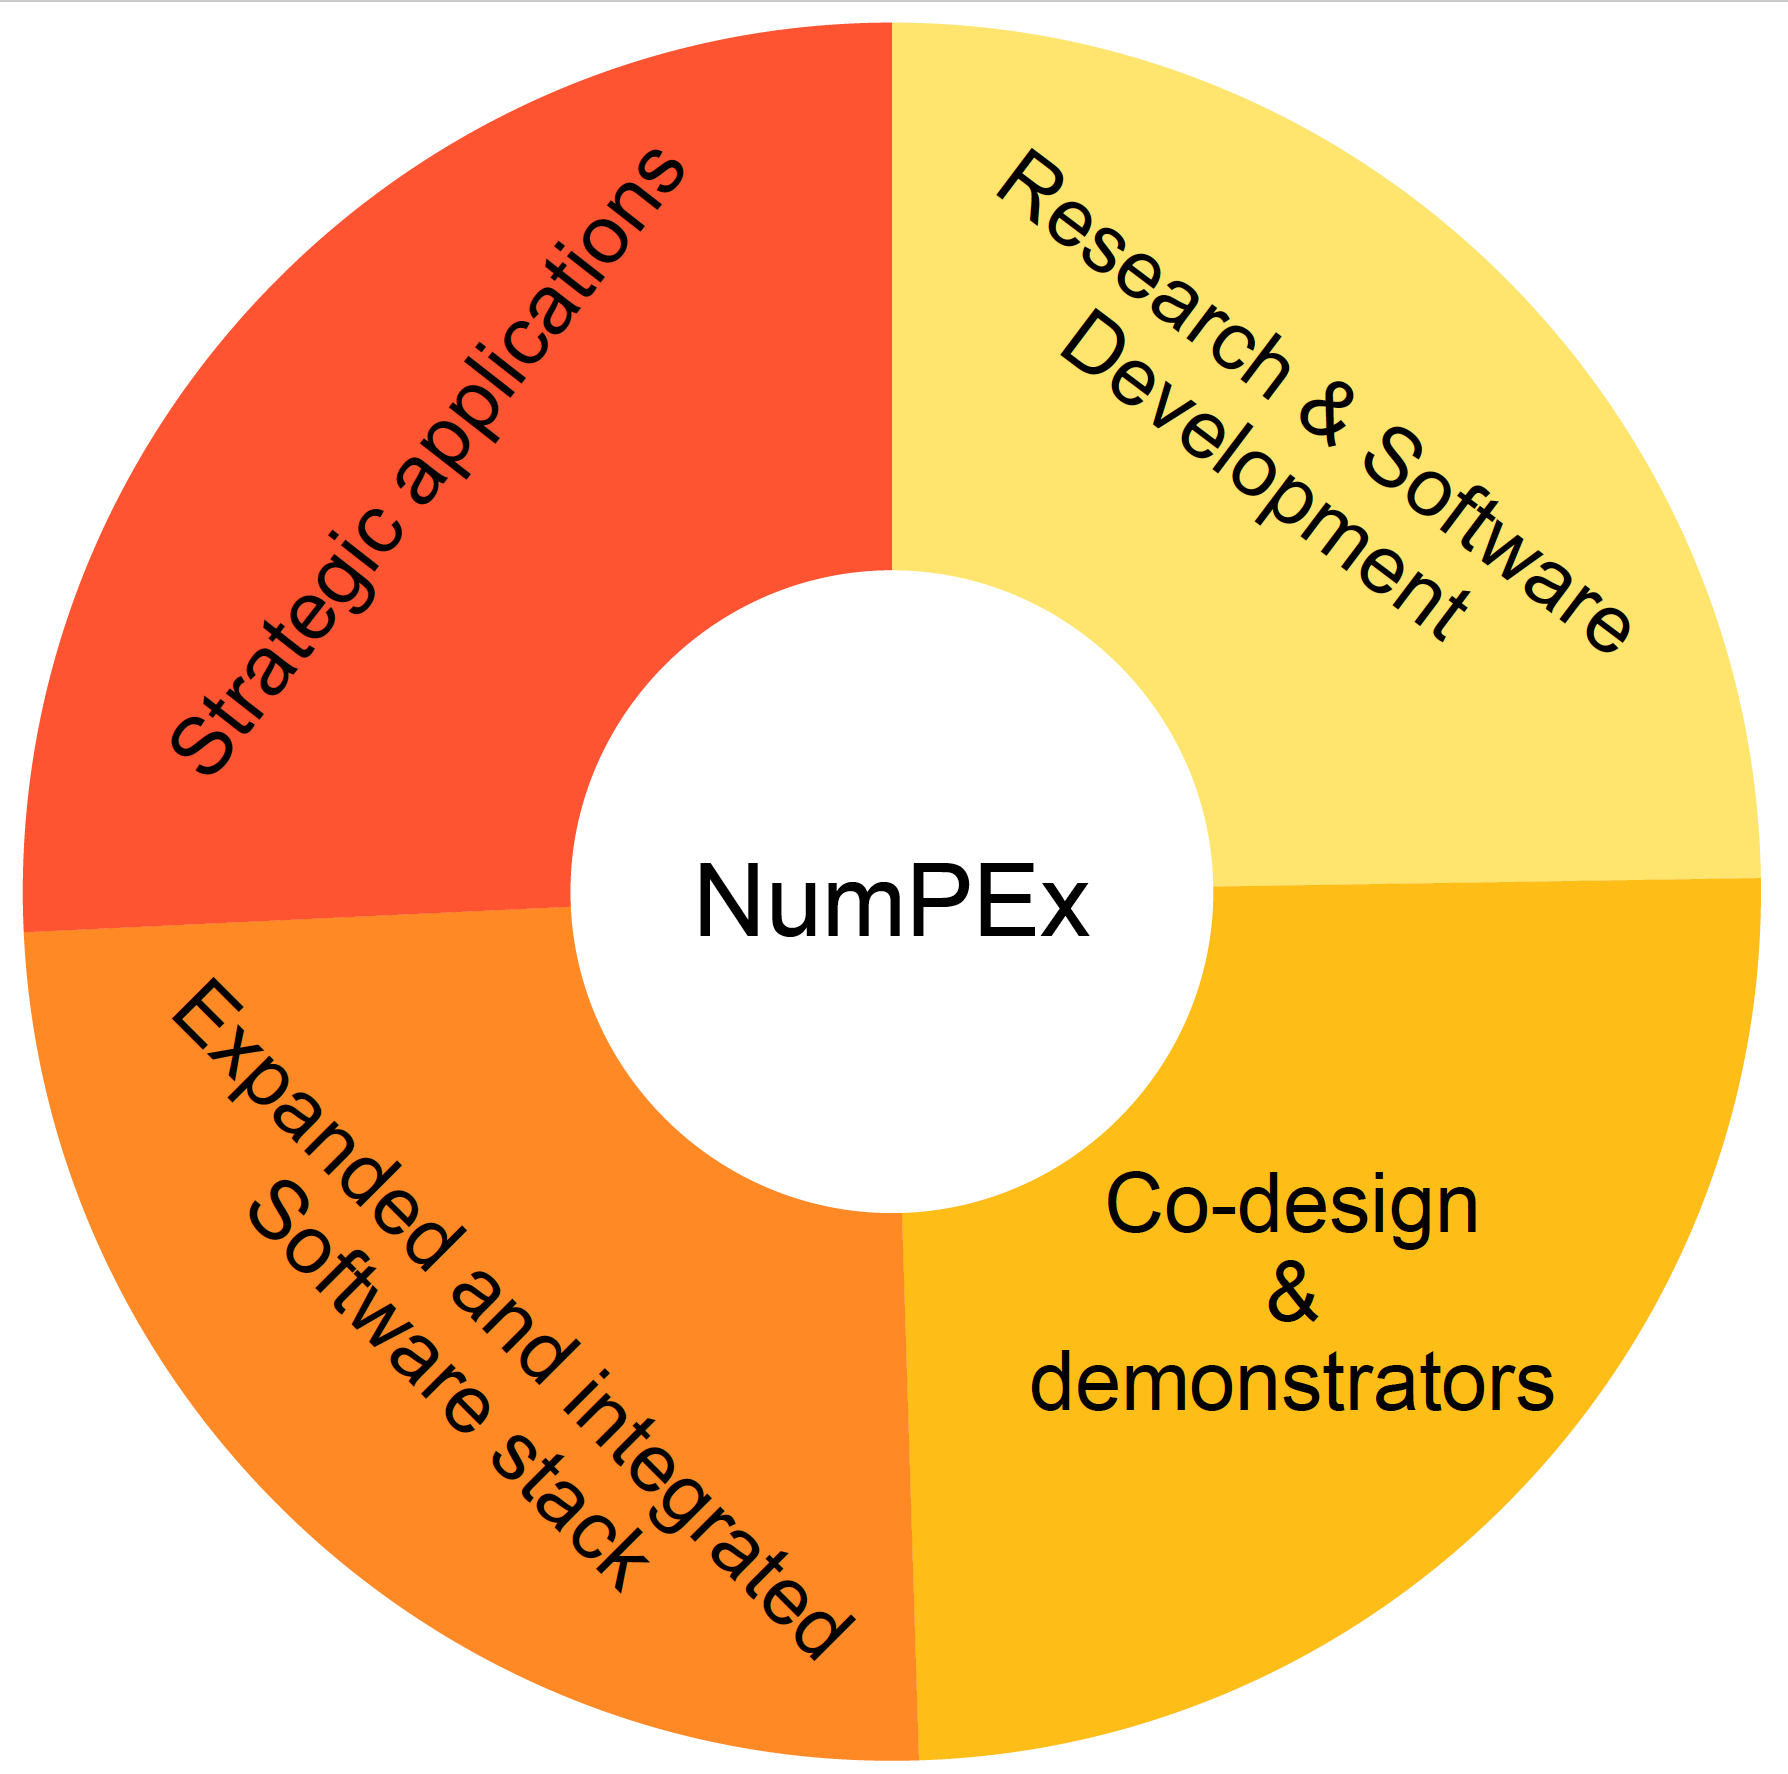
\includegraphics[width=\textwidth]{../figures/numpex-objectives.png}
    \end{column}
  \end{columns}

\end{frame}

\subsection{PC123}

\begin{frame}
  \frametitle{\insertsectionhead}
  \framesubtitle{\insertsubsectionhead}
  \begin{columns}
    \begin{column}{0.5\textwidth}
      \begin{alertblock}{PC<n>\footnote{PC Projet ciblé $\equiv$ IP Integrated project}}

      \begin{enumerate}
        \item \alert{PC1} \textbf{Methods and algorithms for
        Exascale}
        \item \alert{PC2} \textbf{HPC software and tools for the
        Exascale}
        \item \alert{PC3} \textbf{Data-oriented software and tools
        for the Exascale}
      \end{enumerate}
              
    \end{alertblock}
    \end{column}
    \begin{column}{.5\textwidth}
      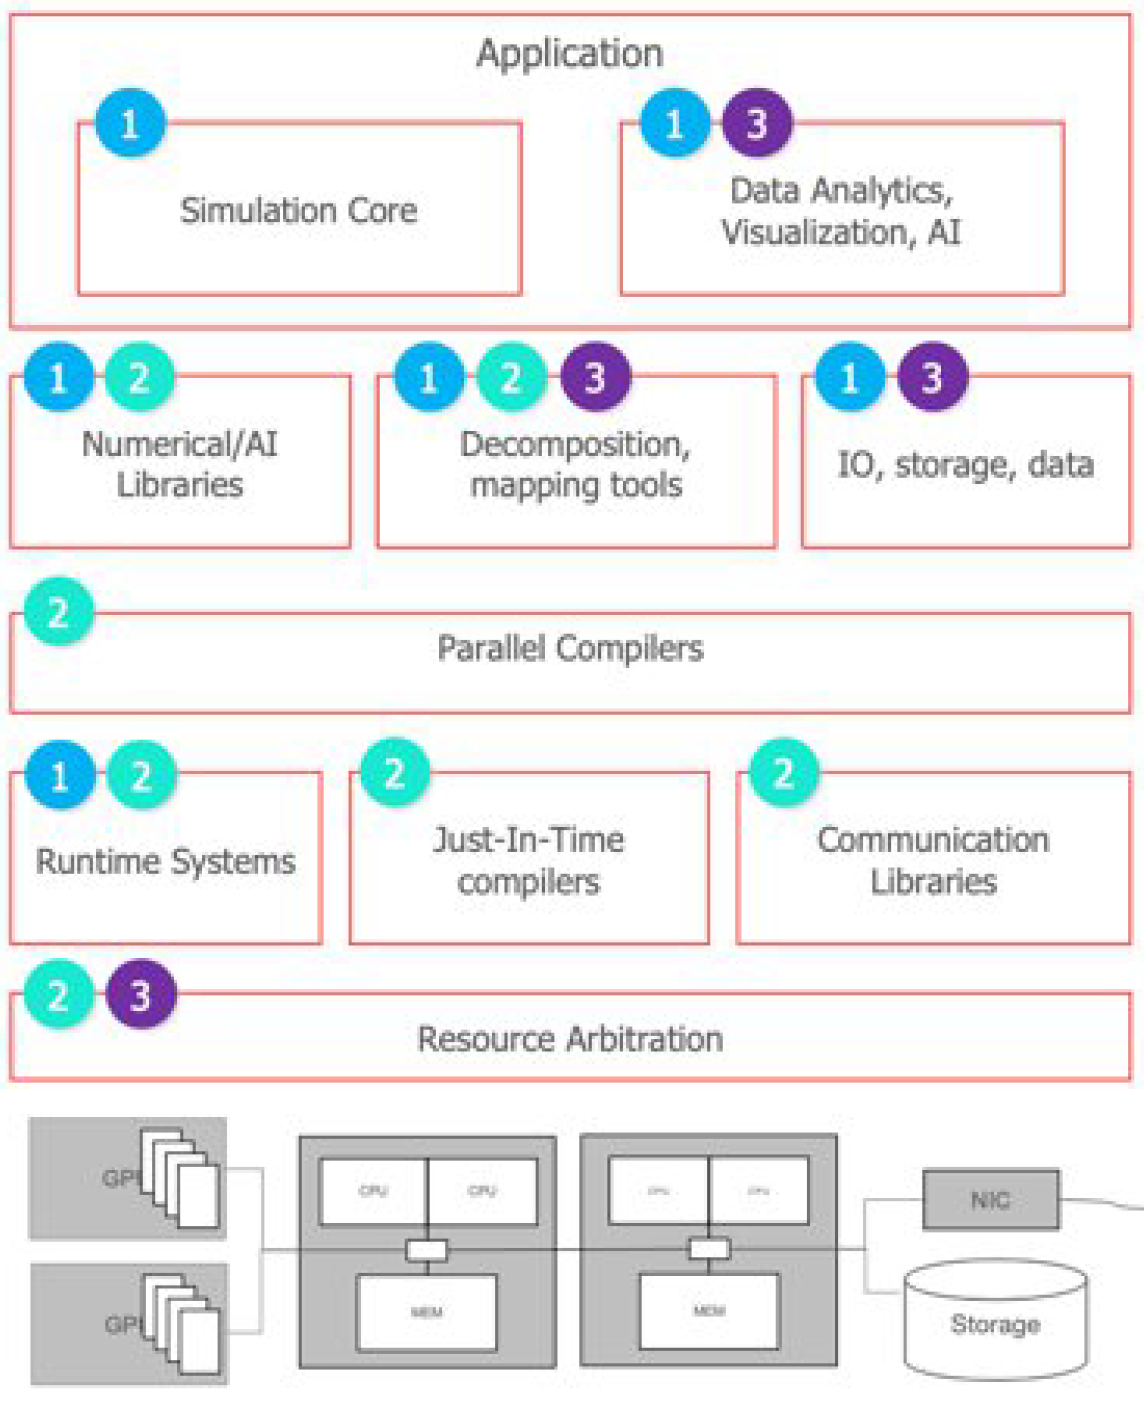
\includegraphics[height=.76\paperheight]{../figures/numpex-ip123.png}
    \end{column}
  \end{columns}
  
\end{frame}
\subsection{PC4}

\begin{frame}
  \frametitle{\insertsectionhead}
  \framesubtitle{\insertsubsectionhead}

  \begin{columns}
    \begin{column}{0.5\textwidth}
      \begin{alertblock}{Wide-area exascale workflows and
        architecture}
        \begin{itemize}
          \item Data logistic between data sources
          (e.g. large scientific instruments) and
          the Exascale system
          \item Cybersecurity and environmental
          sustainability focus
          \item Promoting EU technology (e.g. Atos
          data node and edge servers)
        \end{itemize}
      \end{alertblock}
      
    \end{column}
    \begin{column}{.5\textwidth}
      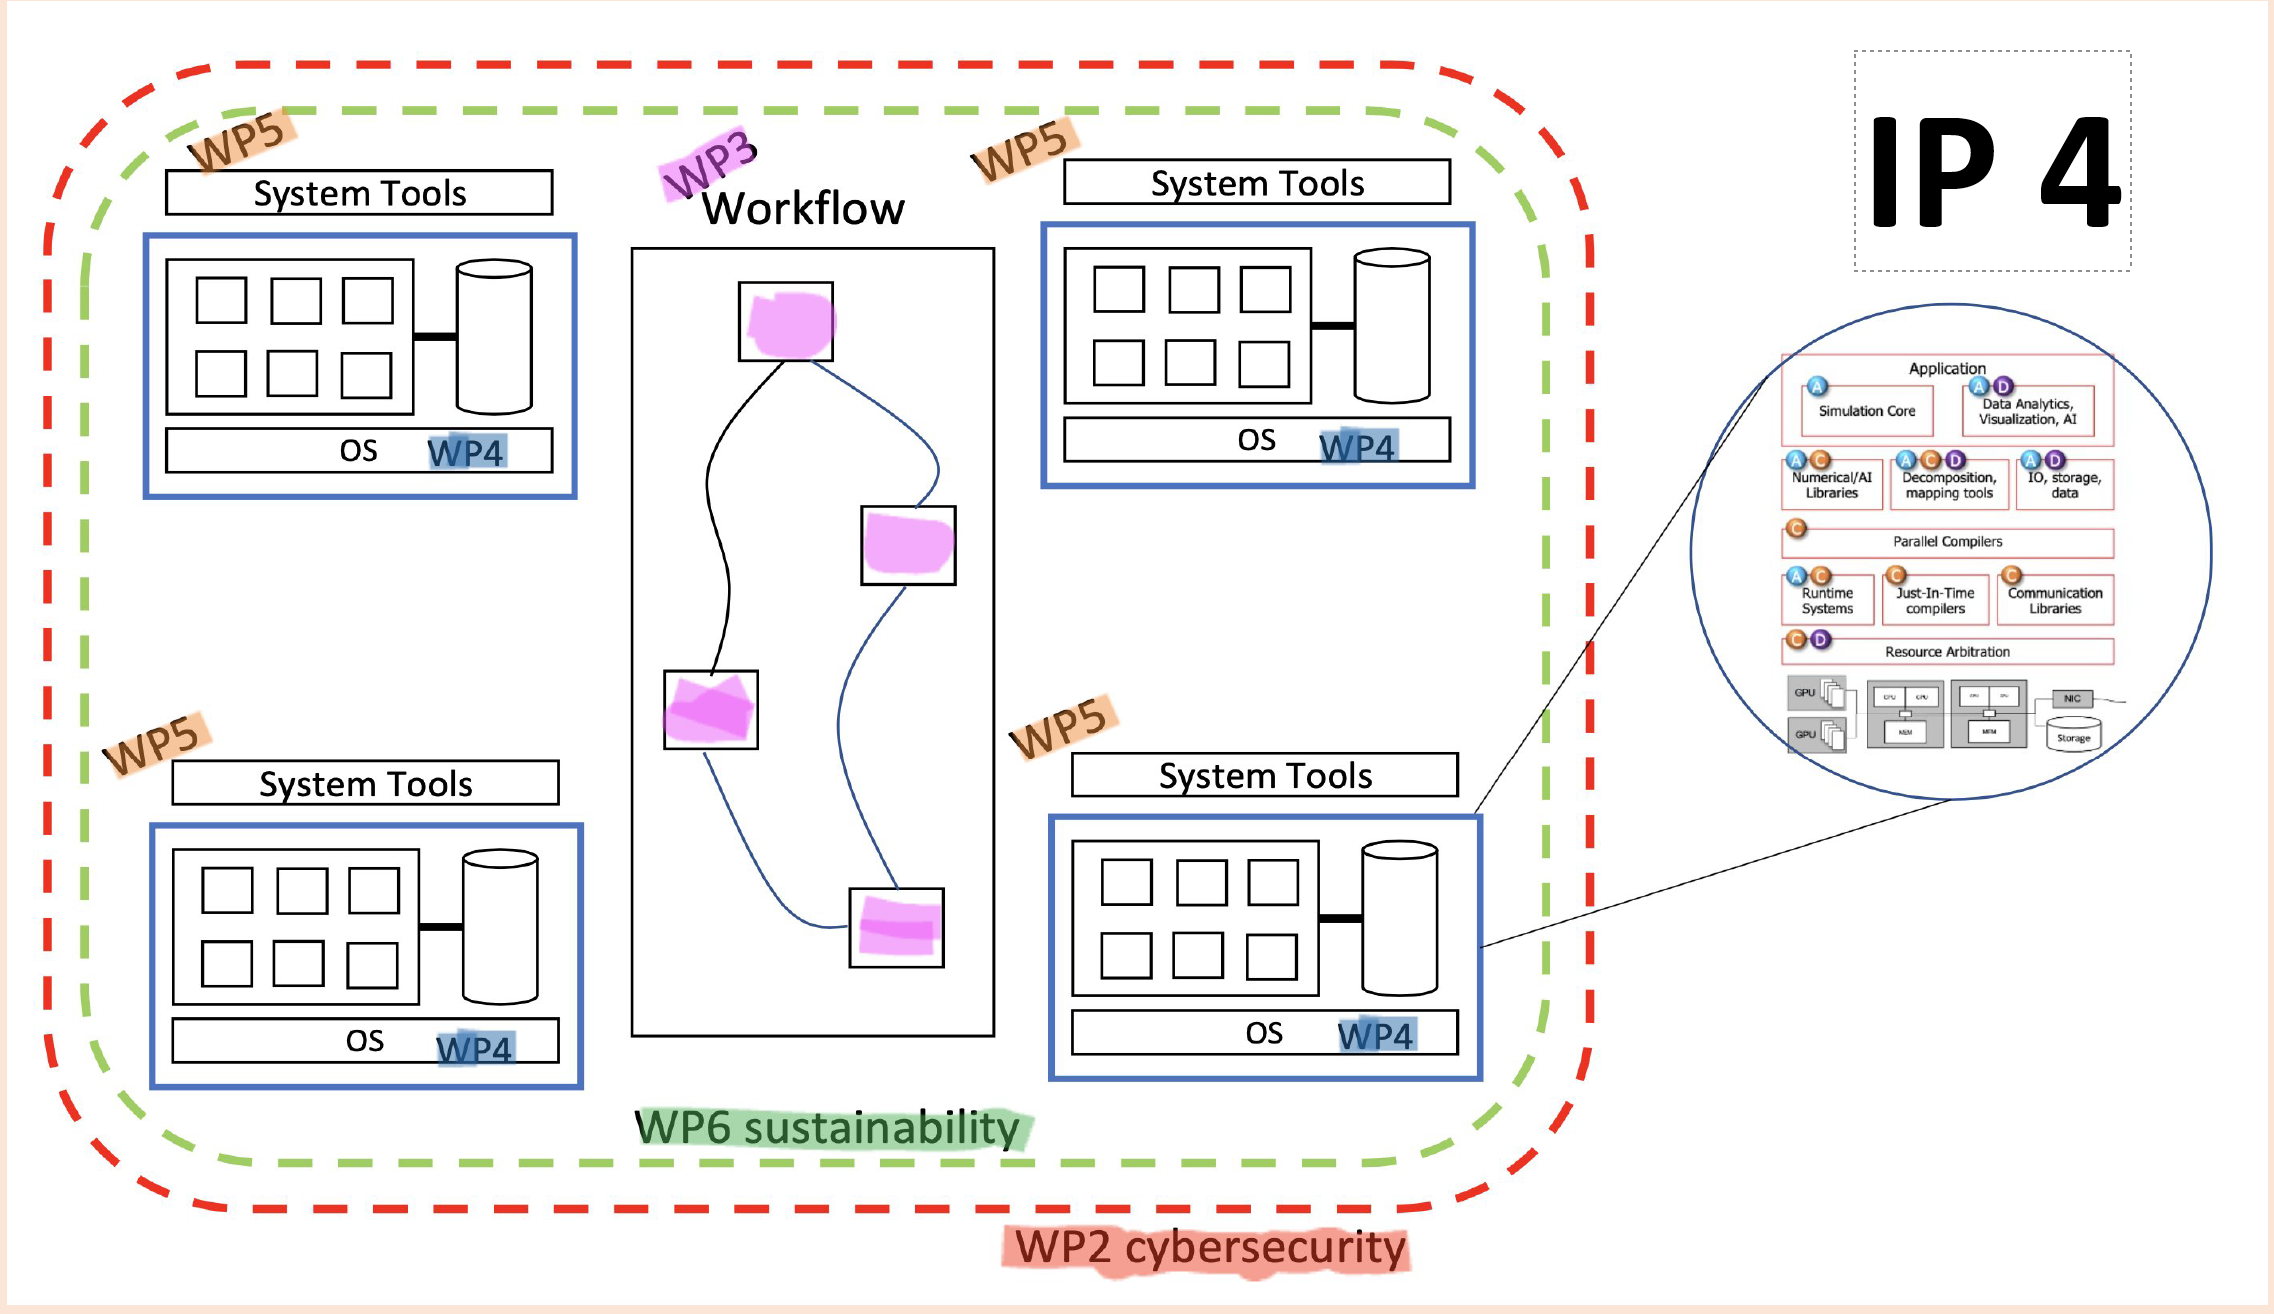
\includegraphics[width=\textwidth]{../figures/numpex-ip4.png}
    \end{column}
  \end{columns}

\end{frame}


\subsection{PC5}

\begin{frame}
  \frametitle{\insertsectionhead}
  \framesubtitle{\insertsubsectionhead}
  \begin{columns}
    \begin{column}{0.5\textwidth}
      \begin{alertblock}{IP 5: Co-design development, software productivity, and demonstrators}
      \begin{itemize}
        \item Identify and define co-design motifs across domain demonstrators and NumPeX
        \item Push R\&D demonstrators requirements into software R\&D (IP 1-4)
        \item Push integrated software developments into demonstrators      
      \end{itemize}
      \end{alertblock}
    \end{column}
    \begin{column}{.5\textwidth}
      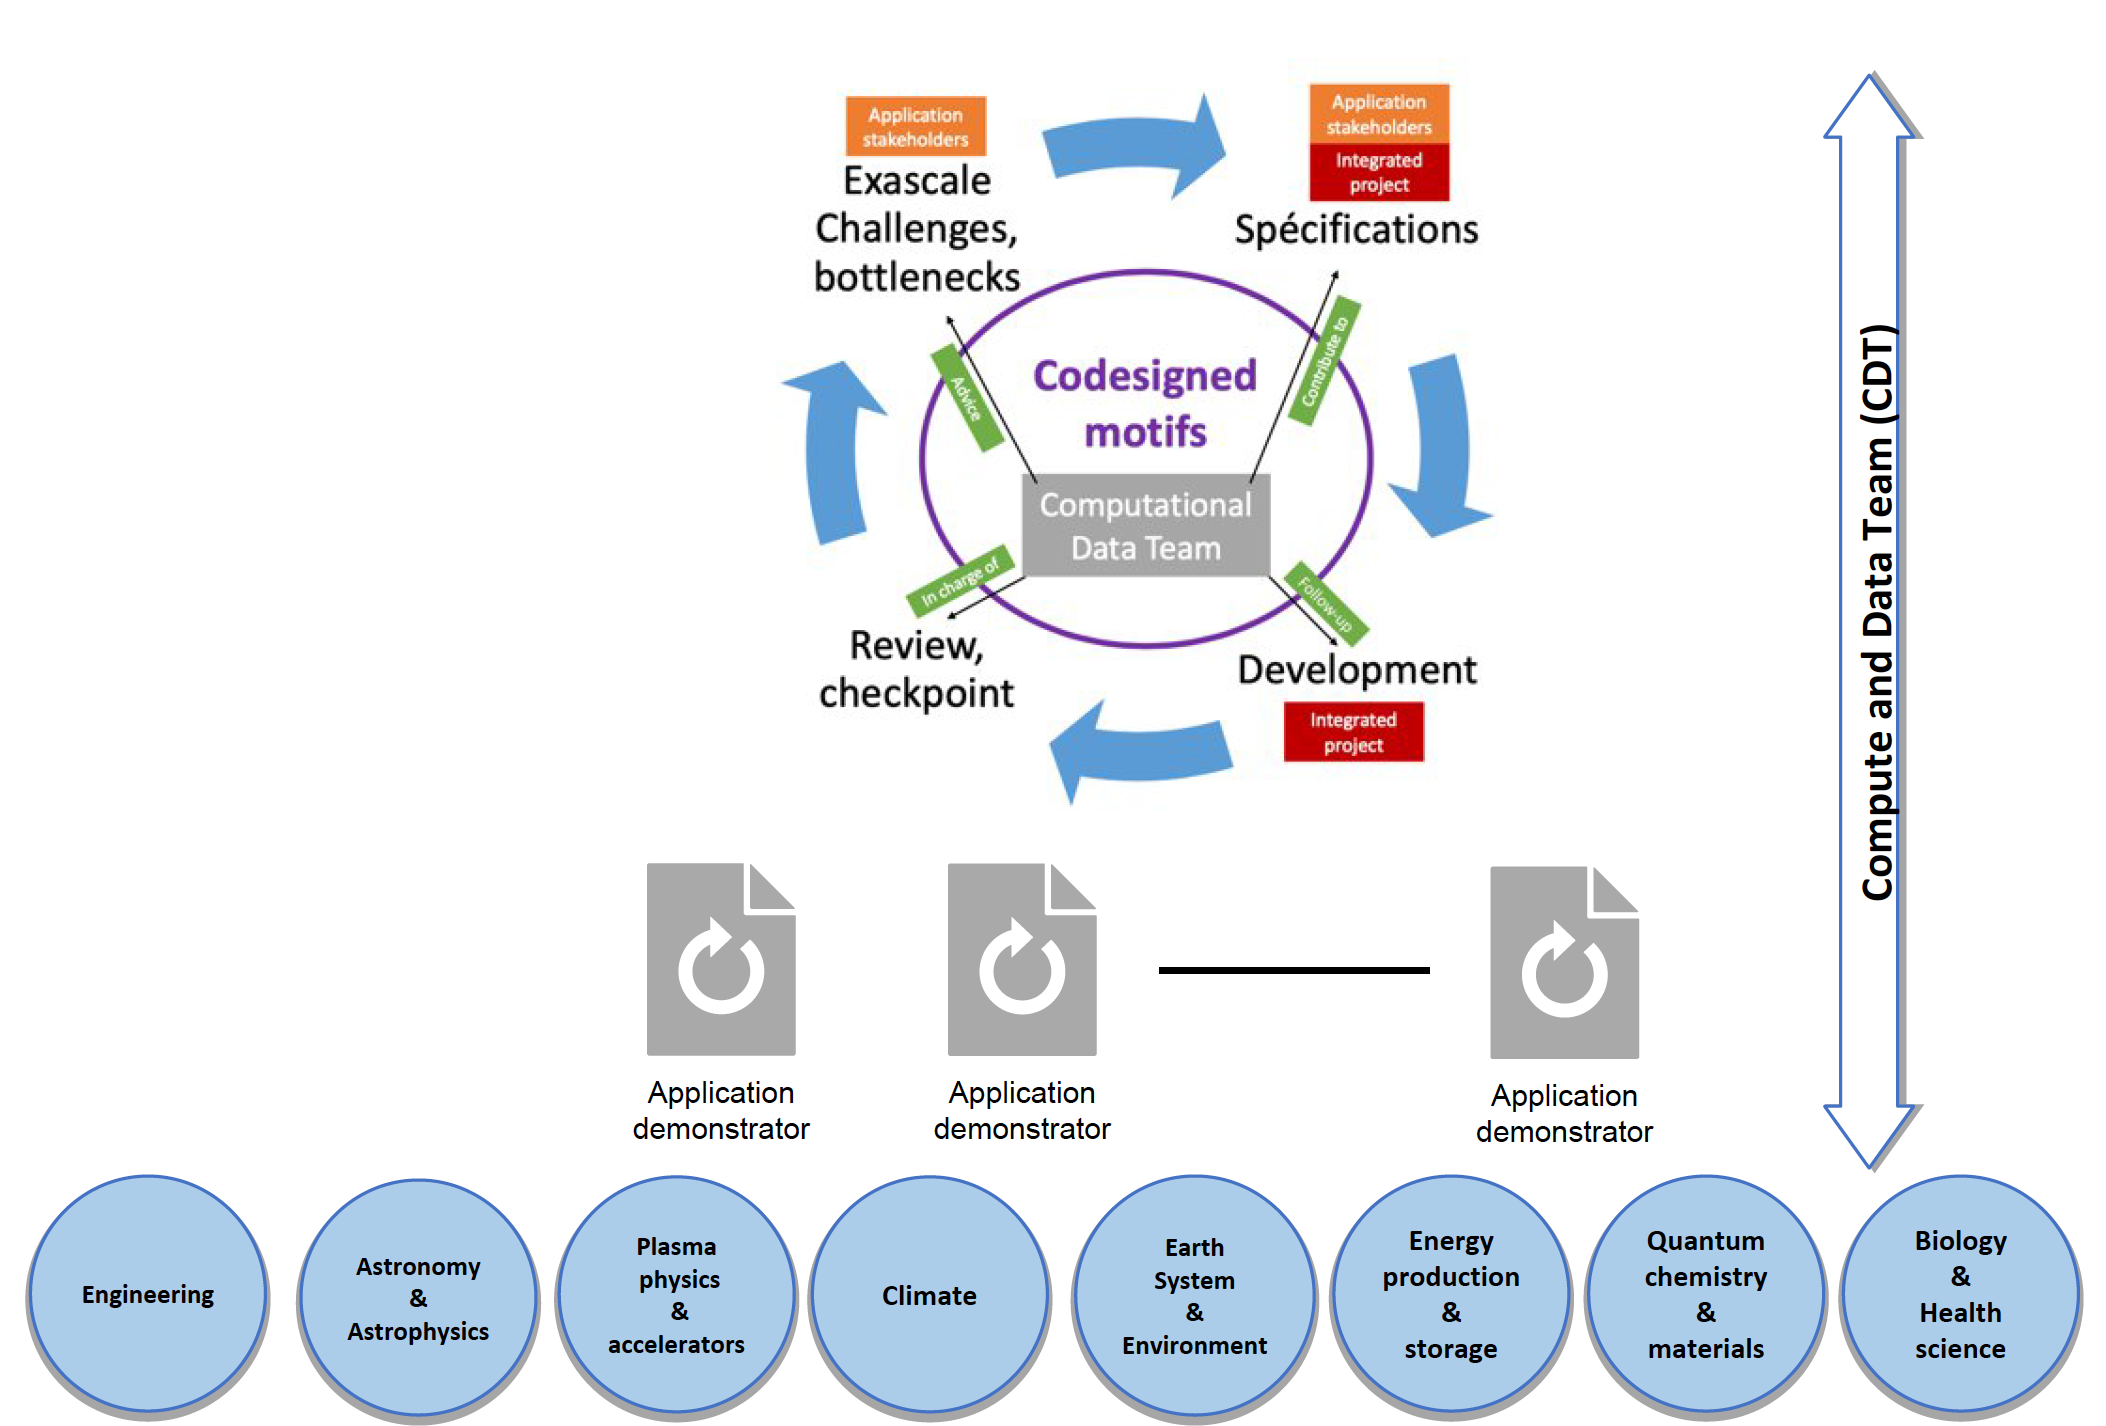
\includegraphics[width=\textwidth]{../figures/numpex-ip5-2.png}
    \end{column}
  
  \end{columns}
\end{frame}
\subsection{NumPEx Software Integration and Productivity}
\begin{frame}
  \frametitle{\insertsectionhead}
  \framesubtitle{\insertsubsectionhead}

  \begin{columns}[t]
    \begin{column}{.5\textwidth}
       \begin{figure}[ht]%
         \centering
          \begin{subfigure}{.45\textwidth}\centering
            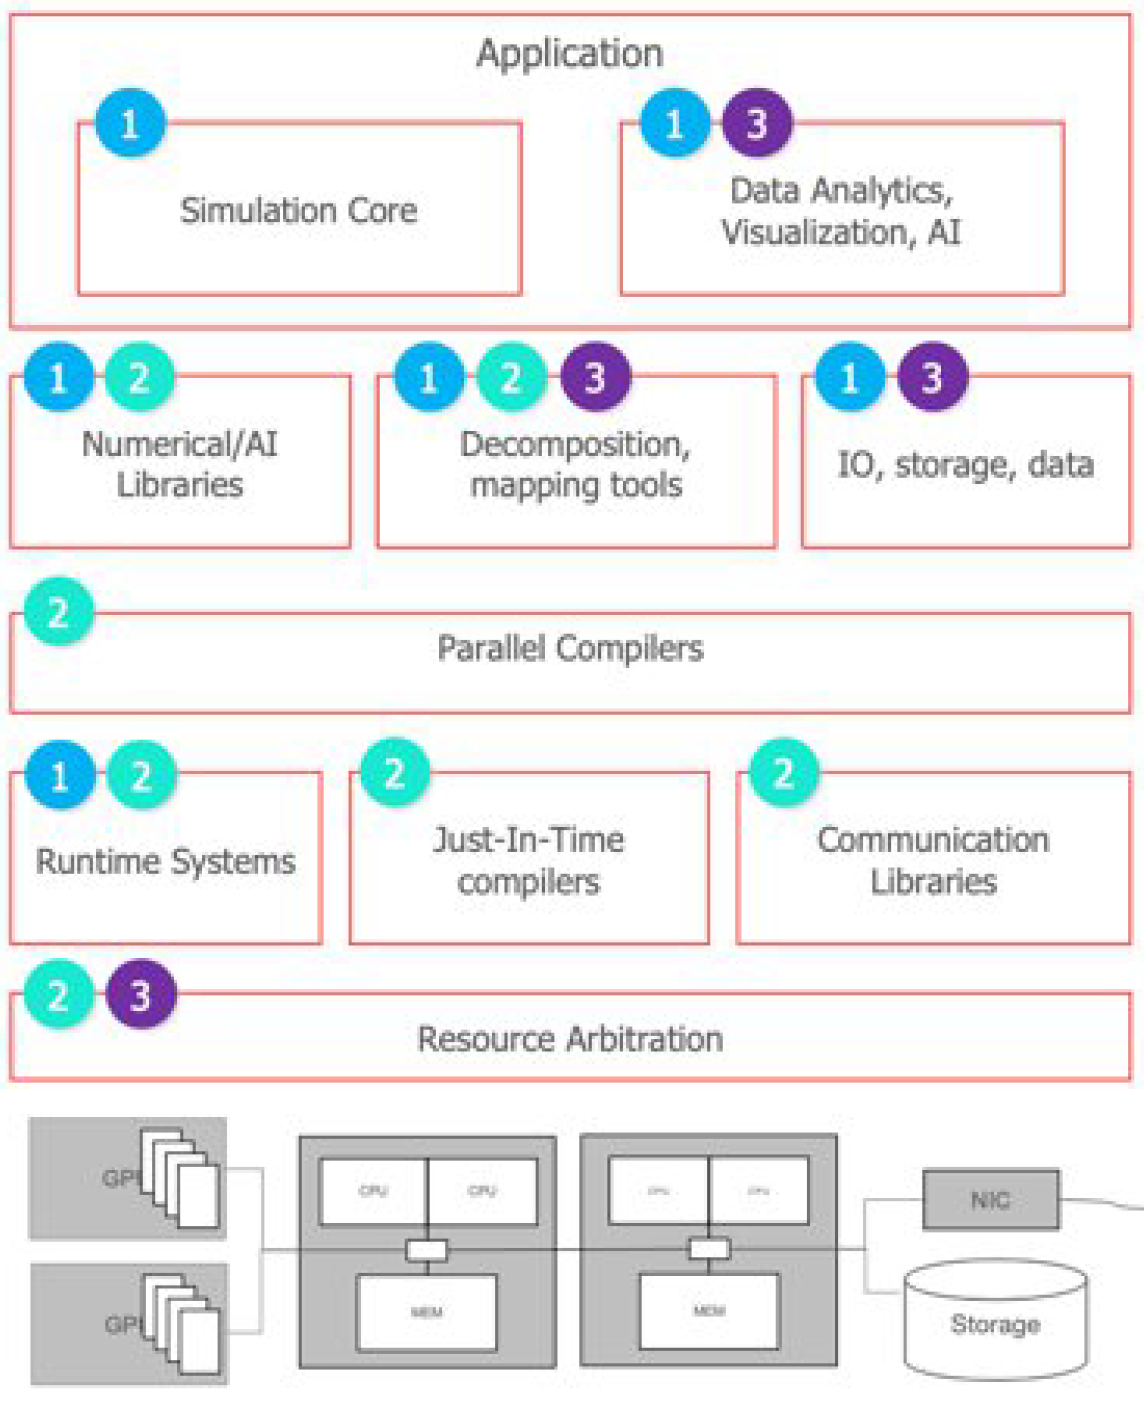
\includegraphics[height=0.5\textwidth]{../figures/numpex-ip123.png}
            \caption{PC1-3}
          \end{subfigure}          
          \begin{subfigure}{.5\textwidth}\centering
            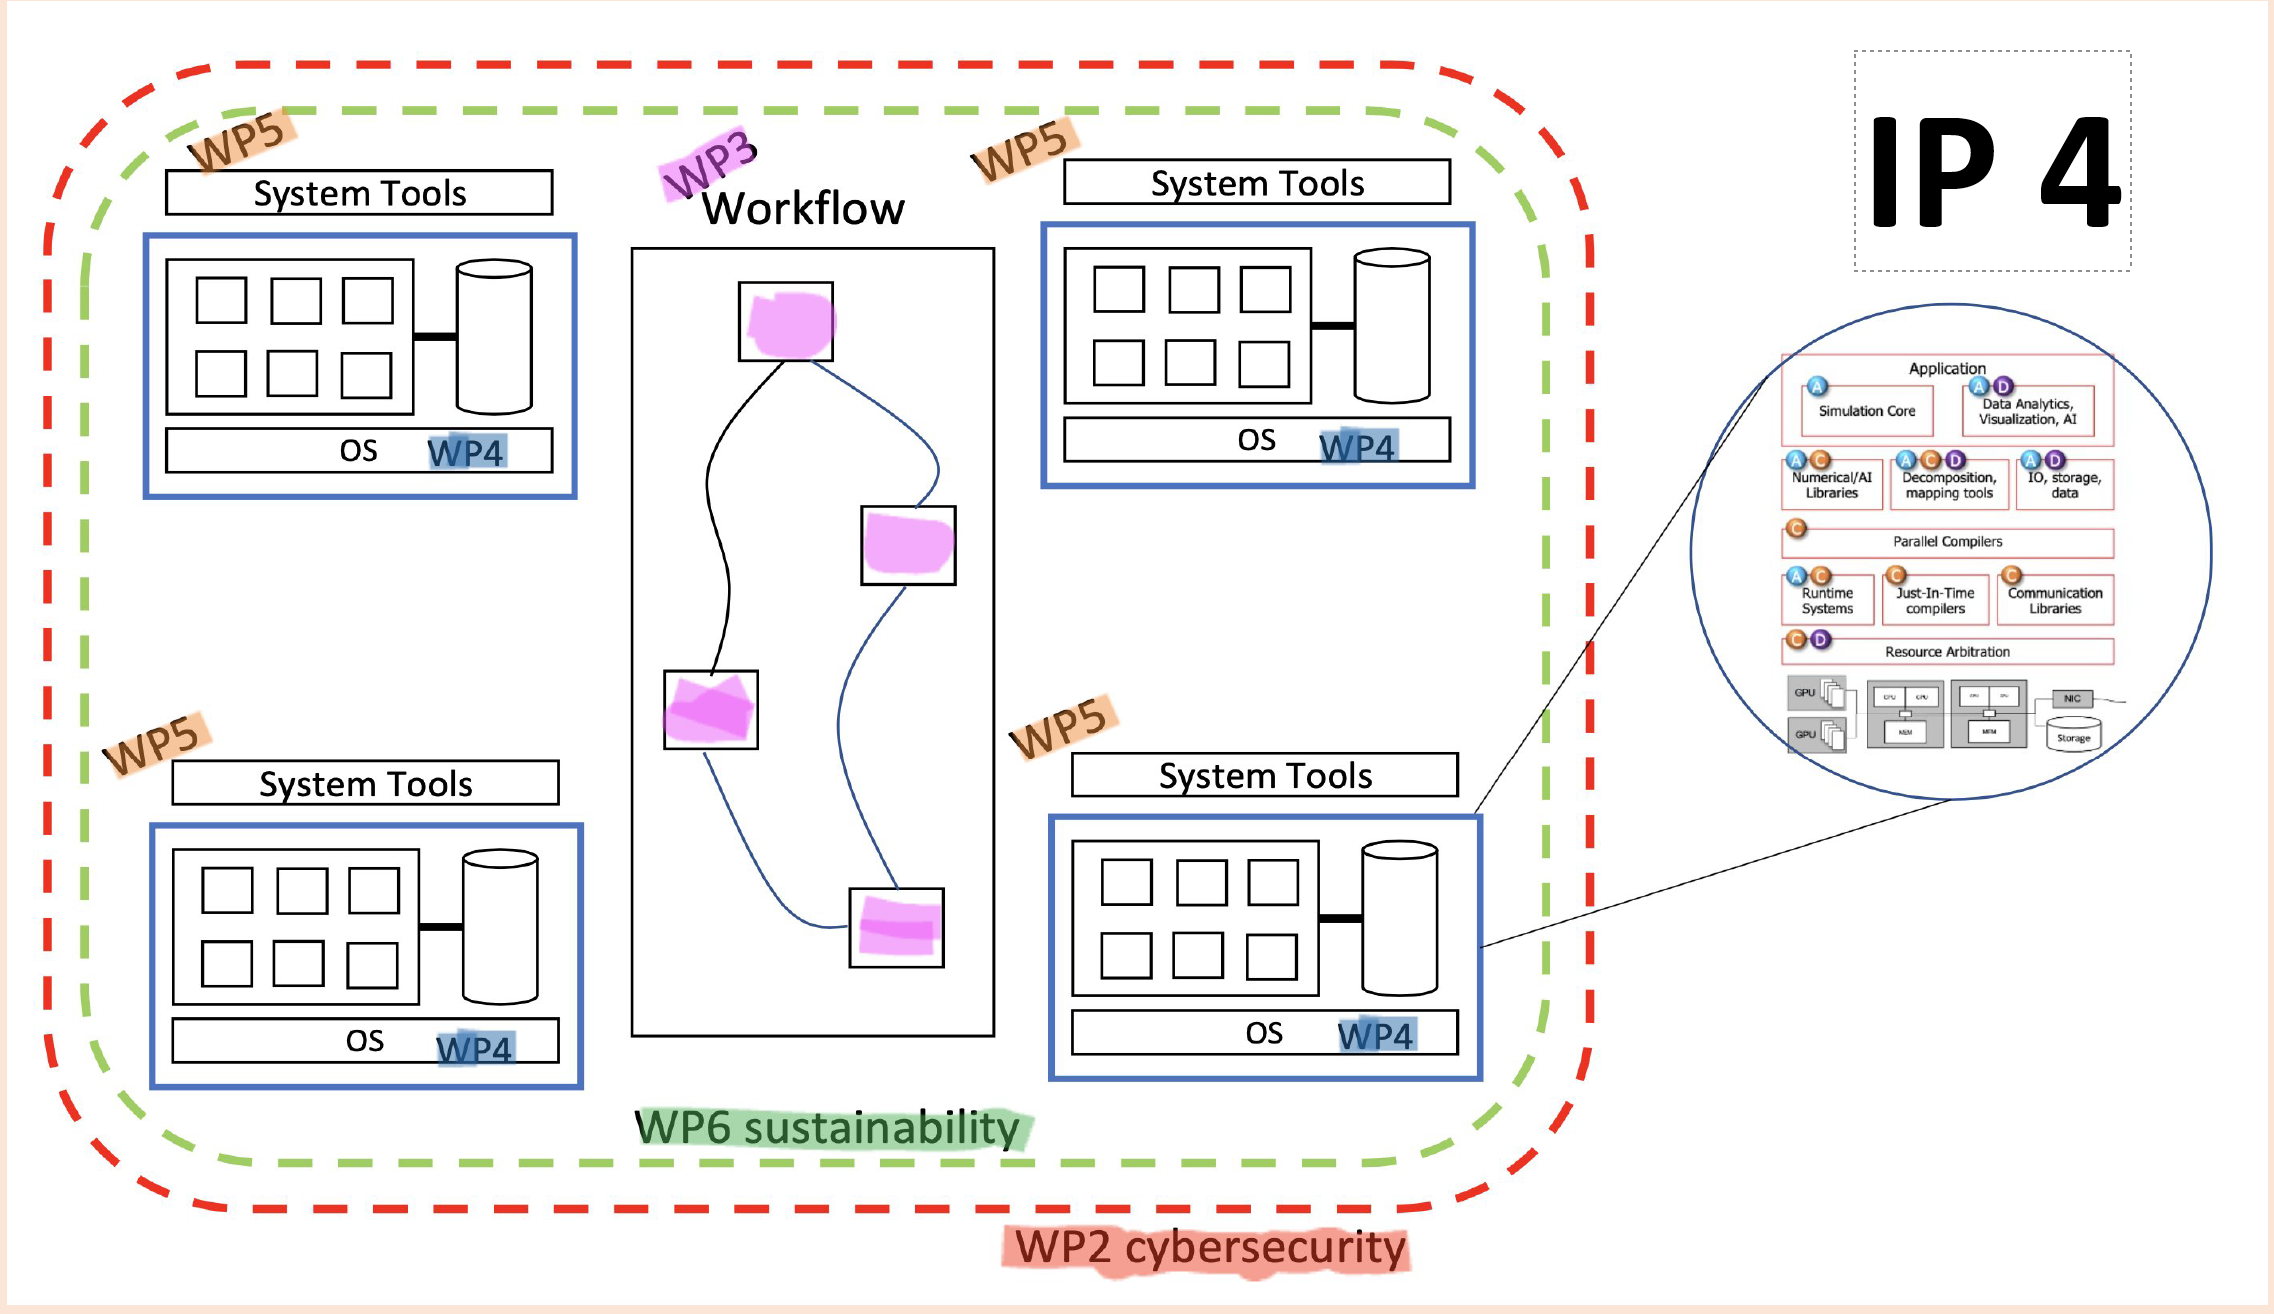
\includegraphics[width=.9\textwidth]{../figures/numpex-ip4.png}
            \caption{PC4}
          \end{subfigure}
          \newline
           \begin{subfigure}{.9\textwidth}\centering
            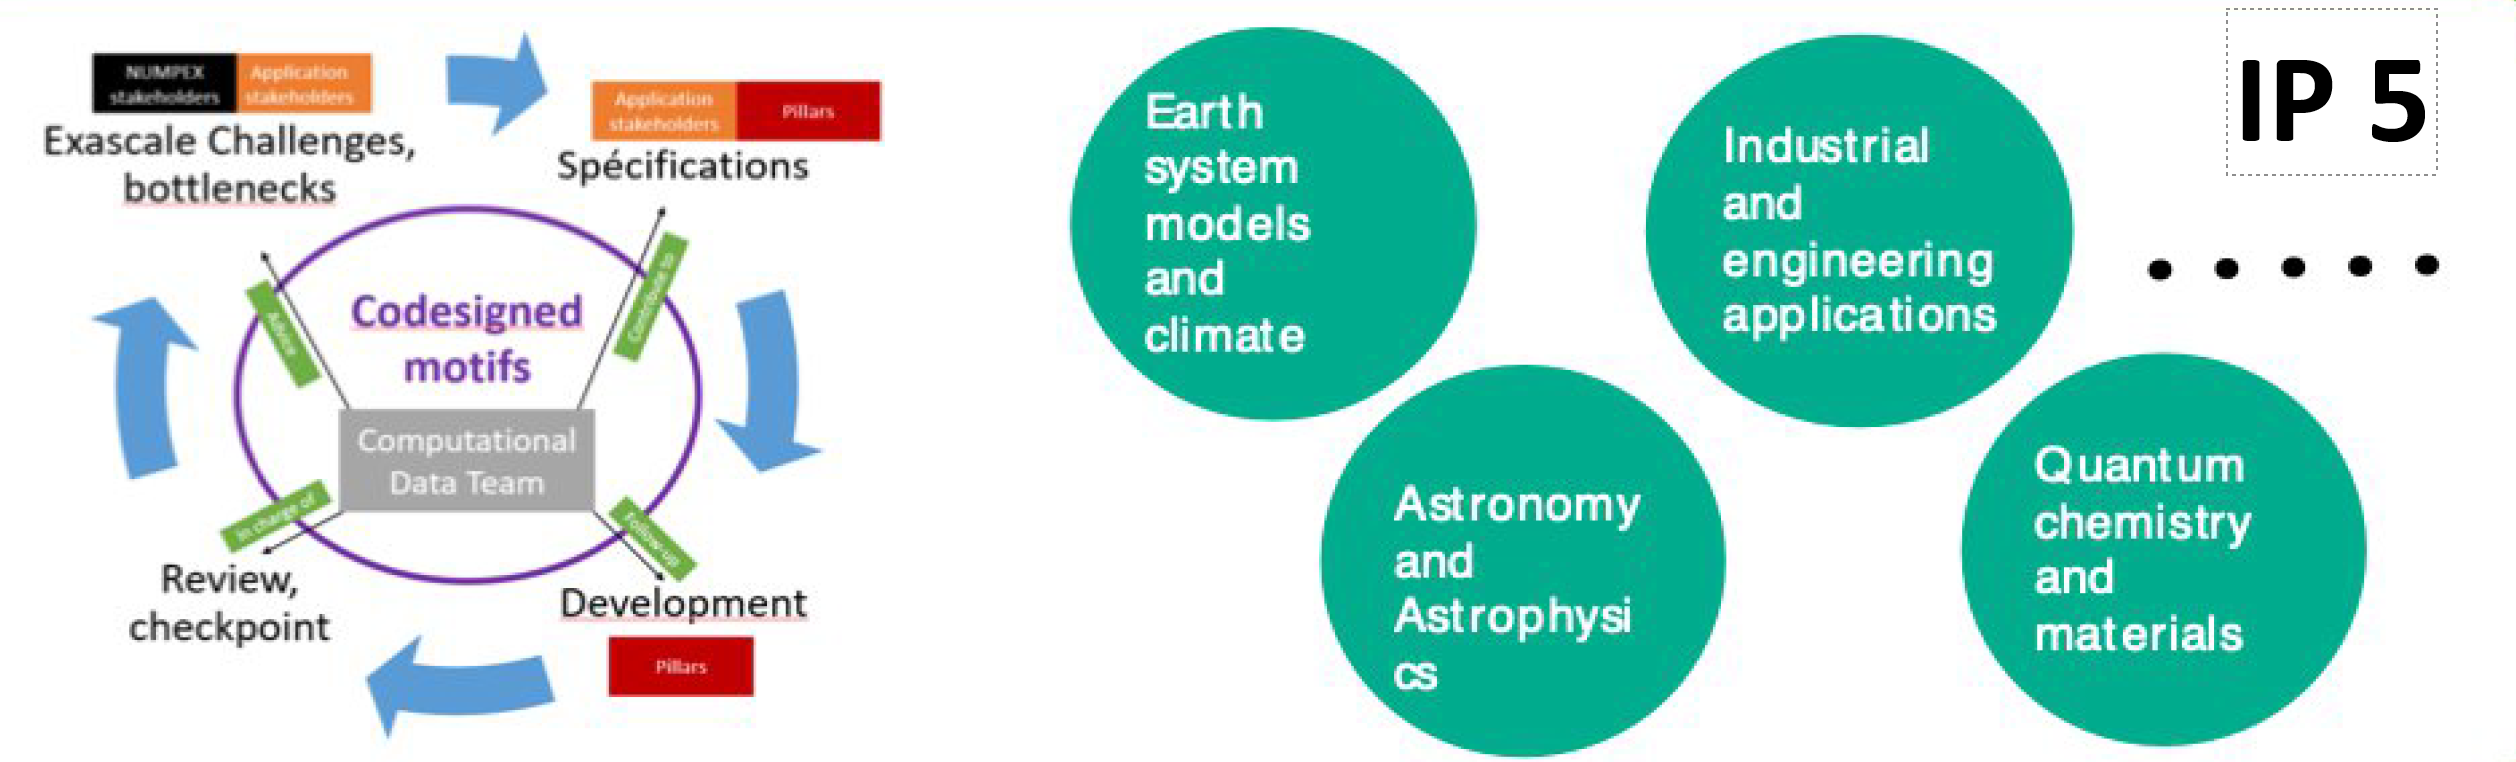
\includegraphics[width=\textwidth]{../figures/numpex-ip5-1.png}
            \caption{PC5}
          \end{subfigure}
         \caption{NumPEx Software Development Kit (SDK)}%
         \label{some-label}%
        \end{figure}
    \end{column}
    \begin{column}{0.5\textwidth}
       \begin{alertblock}{NumPEx Exascale Scientific Software Stack (NE3S)}
         \begin{itemize}
           \item Robust (tested, CI)
           \item Packaged and deployable
           \item Documented, open source, bug          tracking, user forums
           \item Hardware portable (processors,  accelerators)
           \item Interoperable
         \end{itemize}
       \end{alertblock}
    \end{column}
    
    \end{columns}


\end{frame}
%==============================================
\begin{frame}{\insertsectionhead}
  \framesubtitle{ExaMA}
  NUMPEX/ExaMa concentrates on the exascale aspects of the numerical methods, ensuring their scalability to existing and forthcoming hardware.
  \vfill
  Leaders: C Prud'homme \& H Barucq
  \begin{itemize}
    \item 5 Work packages
    \item wide range of topics: 
    \begin{itemize}
        \item Modeling and discretize
        \item Linear, multi-linear and coupled solvers at Exascale
        \item Combine data and  models at Exascale
        \item Optimize and quantify uncertainties at Exascale
    \end{itemize}
    \item Demonstrators through mini-apps will be used to verify the properties of the methods and algorithms developed.
  \end{itemize}
\end{frame}

\subsection{initial Working Group}
\begin{frame}{\insertsectionhead} 
  \framesubtitle{\insertsubsectionhead}
   \begin{itemize}
    \item 10 persons in initial work groups
    \item Other teams consulted on various topics 
    \item Initial Budget: 7 Mio Euros, now a bit more than 6Mio Euros
\end{itemize} 
\end{frame}

%==============================================
\section{Presentation of ExaMA}
%==============================================

\subsection{Identified Bottlenecks/Challenges}

\begin{frame}
  \frametitle{\insertsectionhead}
  \framesubtitle{\insertsubsectionhead}
  \footnotesize
  \begin{columns}
    \column{.5\textwidth}
    \begin{itemize}
      \item (C1) Reduce carbon (GHG) footprint in transportation, buildings, and cities
       \item (C2) Design, control, and manufacture of advanced materials
       \item (C3) Understand and simulate the human brain
       \item (C4) Understand fission and fusion reactions and design advanced experiment facilities for fusion
             \end{itemize} 
    \column{.5\textwidth}
    \begin{itemize}
      \item (C5) Monitor the health of our planet: climate prediction, impact assessment of environmental policies, rapid environmental hazards

        \item (C6) Monitor and personalize the health of human beings 
       \item (C7) Design drugs
       \item (C8) Design cost-effective renewable energy resources: batteries, biofuels, solar photovoltaics
       \item (C9) Understand the Universe
     \end{itemize} 
  \end{columns}

\end{frame}

\begin{frame}[fragile=singleslide]{\insertsectionhead}
  \framesubtitle{\insertsubsectionhead}
  \footnotesize
  \begin{columns}[]
    \begin{column}{.5\linewidth}
      \begin{itemize}
        \item (B1) Energy efficiency
        \item (B2) Interconnect Technology
        \item (B3) Memory technology
        \item (B4) Scalable systems software
        \item (B5) Programming systems
        \item (B6) Data Management
        \item (B7) Exascale Algorithms
      \end{itemize}
    \end{column}
    \begin{column}{.5\linewidth}
      \begin{itemize}
        \item (B8) Discovery, design, and decision algorithms
        \item (B9) Resilience, robustness and accuracy
        \item (B10) Scientific productivity
        \item (B11) Reproducibility, replicability of computation
        \item (B12) Pre/Post-processing
        \item (B13) Integrate Uncertainties
      \end{itemize}
    \end{column}
  \end{columns}

  
\end{frame}

\subsection{WP1: Modeling and Discretization}
\begin{frame}
  \frametitle{\insertsectionhead}
  \framesubtitle{\insertsubsectionhead}

  \begin{columns}
    \column{.5\textwidth}
    \begin{itemize}
      \item Geometric representation and their discrete counterparts [B2, B6, B7, B9, B11-B13] 
      \item physics-based models[B7, B10] 
      \item AI-driven, data-driven, reduced-order, and more generally surrogate models[B2, B7, B8, B10-B13]
      \item Multi-fidelity models [B2, B7, B8]
    \end{itemize}
    \column{.5\textwidth}

    \begin{alertblock}{Persons Involved}
      VF, MM, SL, 
    \end{alertblock}
    \begin{alertblock}{Proposition}
    \begin{itemize}
      \item Extract AI-driven, data-driven, reduced-order, and more generally surrogate models
      \item need to discuss multifidelity
    \end{itemize}
  \end{alertblock}


  \end{columns}


\end{frame}

\subsection{WP2: Linear, Multi-linear and Coupled Solvers at Exascale}
\begin{frame}
  \frametitle{\insertsectionhead}
  \framesubtitle{\insertsubsectionhead}
  \begin{columns}
    \column{.5\textwidth}
    \begin{itemize}
      \item Acceleration techniques for subspace-based methods [B1, B2, B5, B7, B9-B10].
      \item High dimensional problems [B1, B2, B5, B7, B10] 
      \item Randomization [B1, B2, B7, B10]
      \item Exploiting data-sparsity and multiple precision [B1, B2, B5, B7, B10]
      \item Adaptive solution strategies for exascale multiphysical and multiscale models [B7, B9-B11] 
    \end{itemize}
    \column{.5\textwidth}
    \begin{alertblock}{Persons Involved}
      LG, LGi, IR,...  
    \end{alertblock}
    \begin{alertblock}{Proposition}
    \begin{itemize}
      \item need to include computer algebra people
      \end{itemize}
  \end{alertblock}
  \end{columns}

\end{frame}

\subsection{WP3: Combine data and models at Exascale }
\begin{frame}
  \frametitle{\insertsectionhead}
  \framesubtitle{\insertsubsectionhead}
  \begin{columns}
    \column{.5\textwidth}
    [B2, B6, B7, B8, B13]
    \begin{itemize}
      \item Deterministic methods
      \item Stochastic methods
      \item Observations
      \item Taking advantage of multi-fidelity modeling
    \end{itemize}
    \column{.5\textwidth}
    \begin{alertblock}{Persons Involved}
      AV, MA 
    \end{alertblock}
    \begin{alertblock}{proposition}
      \begin{itemize}
        \item add Inverse Problem to WP 3 (currently in WP 4)
      \end{itemize}
    \end{alertblock}
  \end{columns}
\end{frame}

\subsection{WP4: Optimize and quantify uncertainty at Exascale }
\begin{frame}
  \frametitle{\insertsectionhead}
  \framesubtitle{\insertsubsectionhead}
  \begin{columns}
    \column{.5\textwidth}
    [B6-B8, B10, B13]
    \begin{itemize}
      \item Optimization 
      \begin{itemize}
        \item shape, dynamic shape optimization
        \item combinatorial optimization
        \item policy based optimization
        \item automated learning/AI for advanced design
      \end{itemize}
      \item Uncertainty quantification including 
      \begin{itemize}
        \item uncertainty propagation
        \item sensitivity analysis
        \item robust inversion
        \item UQ at different scales
        \item weak vs strong UQ
      \end{itemize}
    \end{itemize}
    \column{.5\textwidth}
    \begin{alertblock}{Persons Involved}
      JG, YP, ET
    \end{alertblock}
  \end{columns}
\end{frame}
\subsection{WP5: Demonstrate methods and algorithms at Exascale}
\begin{frame}
  \frametitle{\insertsectionhead}
  \framesubtitle{\insertsubsectionhead}

  \begin{columns}
    \column{.5\textwidth}
    [B1-B13]
    \begin{itemize}
      \item Properties Verification on small/mini apps within PC1
      \item Co-design with the CDT and PC5
    \end{itemize}
    \column{.5\textwidth}
    \begin{alertblock}{Persons Involved}
      LGr + ALL
    \end{alertblock}
  \end{columns}

\end{frame}
\subsection{Principles}
\begin{frame}[fragile=singleslide]{\insertsectionhead}
  \framesubtitle{\insertsubsectionhead}

  \begin{itemize}
    \item \textbf{Openness} and \textbf{transparency} of the project 
    \item \textbf{Collaboration} with other projects : 
    \begin{itemize}
      \item 
        co-design with PC5, collaboration with PC2,3,4\
        \item 
          collaboration with other projects e.g. EuroHPC projects(Coe) and other PEPR (IA, Diademe,TRACCS-Météo...
    \end{itemize}
    \item \textbf{Inclusiveness} of the community 
    \begin{itemize}
      \item use the project as leverage for co-funding  or, also, collaborating outside the project eg phd co-advisors
      \item training : initial(train future PhD students) and continuous (broader community)
    \end{itemize}      
  \end{itemize}

\end{frame}

\subsection{Calendrier}
\begin{frame}
  \frametitle{\insertsectionhead}

  \begin{itemize}
    \item Project proposal by the end of year with inter PC discussion as well as external partners
    \item End of year/March 2023 discussion with ANR, Contracting,...
    \item Project start in March/April 2023 (in sync with other PCs)
    \item Total duration : 5 years (+18 months)
  \end{itemize}

  \begin{alertblock}{Oct 20}
    Next Global Meeting INRIA Paris
  \end{alertblock}
\end{frame}

\subsection{Organisation}

\subsection{Project Management}
\begin{frame}
  \frametitle{\insertsectionhead}
  \framesubtitle{\insertsubsectionhead}

  \begin{itemize}
    \item Several co-leads per WP 
    \item Meeting every 2 or 3 weeks to advance the writing
    \item Use of Google Doc and GitHub (repo and project management)
  \end{itemize}

\end{frame}


